\documentclass[final,5p,times,twocolumn,authoryear,11pt]{elsarticle}

\usepackage[spanish]{babel}
\usepackage{amssymb}
\usepackage{amsmath}
\usepackage{graphicx}
\usepackage{booktabs}
\usepackage{float}
\usepackage{url}
\usepackage{algorithm}
\usepackage{algpseudocode}

\graphicspath{{figuras/}}
\raggedbottom
\renewcommand{\algorithmicrequire}{\textbf{Entrada:}}
\renewcommand{\algorithmicensure}{\textbf{Salida:}}
\floatname{algorithm}{Algoritmo}

\journal{Métodos Numéricos CC2104}

\begin{document}

% ==================== PORTADA DE EVALUACIÓN ====================
\begin{titlepage}
    \centering
    \IfFileExists{logo_utec.png}{
\includegraphics[width=0.35\textwidth]{logo_utec.png} \par}{}
    \vspace{1cm}

    {\Huge \bfseries
Modelamiento numérico transitorio del transporte de calor 1D en el flujo sobre un tubo cilíndrico con difusividad térmica variable
    \par}
    \vspace{2cm}

    {\Large \bfseries Integrantes: \par}
    \vspace{0.5cm}
    \begin{tabular}{ll}
        Calapuja Quispe, Angela Lorena & (202310600) \\
        Dongo Triveño, Daniel Mateo & (202310506)\\
        Hilario Quintana, Jeffry Arturo & (202020082)\\
        Zorrilla Pelaez, María José & (202510379)\\
    \end{tabular}

    \vspace{2cm}

    {\Large \bfseries Métodos Numéricos (CC2104) \par}
    \vspace{0.5cm}
    {\large Profesor: Ponce Cegovia, Roger Ivan \par}

    \vfill

    % COMPLETAR la fecha de entrega
    {\large Fecha de entrega: 18/10/2026 \par}
    \vspace{1cm}
\end{titlepage}

\newpage
\setcounter{page}{1}

% ==================== INICIO DEL PAPER ====================
\begin{frontmatter}

\title{Modelamiento numérico transitorio del transporte de calor 1D en el flujo sobre un tubo cilíndrico con difusividad térmica variable}

\author[utec]{Calapuja Quispe, Angela Lorena}
\ead{angela.calapuja@utec.edu.pe}

\author[utec]{Dongo Triveño, Daniel Mateo}
\ead{daniel.dongo@utec.edu.pe}

\author[utec]{Hilario Quintana, Jeffry Arturo}
\ead{jeffry.hilario@utec.edu.pe}

\author[utec]{Zorrilla Pelaez, María José}
\ead{maria.zorrilla@utec.edu.pe}

\affiliation[utec]{organization={Universidad de Ingeniería y Tecnología},
            city={Lima},
            country={Perú}}

\begin{abstract}
El transporte de calor en fluidos sobre superficies sólidas es relevante en la ingeniería térmica, y se complica cuando la difusividad térmica depende de la temperatura. Este estudio modeló numéricamente el transporte transitorio de calor unidimensional con advección y difusividad variable, con el propósito de analizar el avance del frente de temperatura entre una corriente caliente a 100~\textdegree C y la pared de un tubo cilíndrico a 0~\textdegree C. El espacio se discretizó con diferencias finitas, el tiempo se avanzó con un método de Runge-Kutta diagonalmente implícito de cuarto orden, y la no linealidad y los sistemas lineales de cada etapa se resolvieron con Newton-Raphson y Gauss-Seidel. Se calculó el error máximo frente a una solución de referencia y se variaron el coeficiente de variación de la difusividad, la velocidad del fluido y los pasos espacial y temporal. El esquema convergió en todas las etapas; el caso base tuvo un error máximo de 0,50~\textdegree C y el frente alcanzó 0,909~m en 2,0~s. El error disminuyó al reducir ambos pasos, la velocidad desplazó el frente hacia la pared y el coeficiente de variación lo acercó a la corriente caliente. El costo computacional fue bajo.
\end{abstract}

\begin{keyword}
transporte de calor \sep difusividad térmica variable \sep Runge-Kutta diagonalmente implícito \sep Newton-Raphson \sep Gauss-Seidel
\end{keyword}

\end{frontmatter}

% ==================== CUERPO DEL DOCUMENTO ====================

\section{Introducción}
\label{sec:introduccion}

El transporte de calor en fluidos que se mueven sobre superficies sólidas es un problema central de la ingeniería térmica, con aplicaciones en sistemas de enfriamiento industrial, intercambiadores de calor de tubos y componentes de turbomaquinaria. En estos sistemas, el fluido arrastra la temperatura con su movimiento (advección) y, al mismo tiempo, la temperatura se reparte por conducción (difusión). Además, las propiedades térmicas de los materiales no son constantes: la difusividad térmica cambia con la temperatura, y suponerla constante da una descripción poco realista cuando los cambios de temperatura son grandes \citep{Wang2022, Filipov2023}. Esta dependencia hace que la ecuación del calor sea no lineal y que casi nunca tenga solución exacta, por lo que se recurre a métodos numéricos.

El flujo sobre un tubo cilíndrico en régimen estacionario y transitorio fue estudiado mediante dinámica de fluidos computacional por \citet{Singh2024}. El estudio numérico de la conducción de calor con propiedades que dependen de la temperatura se abordó con distintas técnicas: \citet{Wang2022} propusieron un método de soluciones fundamentales localizado, \citet{Ejaz2024} un algoritmo de colocación para una difusividad térmica no uniforme, \citet{MtAznam2019} wavelets de Haar en problemas de aletas con transferencia de calor no lineal, y \citet{Filipov2023} resolvieron la transferencia de calor transitoria con conductividad que depende de la temperatura mediante una discretización implícita en el tiempo. Para avanzar en el tiempo problemas de convección-difusión, \citet{Deng2014} aplicaron un método de Runge-Kutta diagonalmente implícito, \citet{Levy2022} compararon esquemas de discretización temporal implícitos para métodos de Galerkin discontinuo híbrido y \citet{Deng2015} desarrollaron un método de este tipo, de cuarto orden, para la ecuación de Burgers 1D, que demostraron incondicionalmente estable. \citet{Kennedy2003} construyeron esquemas de Runge-Kutta aditivos para problemas de convección-difusión-reacción, \citet{Ascher1997} formularon métodos Runge-Kutta implícito-explícitos para ecuaciones diferenciales parciales dependientes del tiempo y \citet{Boscarino2015} propusieron métodos de este tipo, linealmente implícitos, para problemas de convección-difusión con difusión degenerada, que solo requieren resolver sistemas lineales. \citet{Bevan2016} compararon formas implícitas y explícitas de un método de paso fraccionado en flujos incompresibles, y el hecho de que un esquema sea implícito o explícito influye en su estabilidad \citep{Butcher1996}. Por último, \citet{Zhang2015} estudiaron la convergencia de los métodos de Gauss-Seidel para sistemas lineales con matrices H generales.

Sin embargo, en la literatura revisada predominan los estudios de conducción no lineal sin un escenario de flujo, y los estudios de métodos implícitos se centran en otras ecuaciones. Por eso hace falta un modelo propio y claro para el transporte transitorio de calor con difusividad variable, que permita medir la precisión, la robustez y el costo de la combinación de un método implícito para avanzar en el tiempo, un método para la no linealidad y un método iterativo para sistemas lineales.

Por ello, el objetivo general de este estudio es modelar numéricamente el transporte de calor transitorio unidimensional con advección y difusividad térmica que depende de la temperatura, con el propósito de analizar cómo avanza el frente de temperatura entre una corriente caliente y la pared de un tubo cilíndrico. Para alcanzar esta meta, se plantean cuatro objetivos específicos: (i) formular e implementar el modelo unidimensional mediante diferencias finitas, el método de Runge-Kutta diagonalmente implícito de cuarto orden (SDIRK4), Newton-Raphson y Gauss-Seidel, y verificar que todas las etapas del esquema convergen; (ii) evaluar el comportamiento del modelo con los parámetros base y condiciones de frontera de Dirichlet, determinando el error máximo de la temperatura frente a una solución de referencia; (iii) analizar la robustez del esquema variando el coeficiente de variación de la difusividad ($\beta$), la velocidad del fluido ($v$) y los pasos espacial y temporal, y determinando el error máximo, las iteraciones y el tiempo de cómputo; y (iv) aplicar el modelo al calentamiento transitorio de una corriente caliente que se acerca a la pared de un tubo cilíndrico a temperatura fija, cuantificando en distintos instantes la posición del frente de temperatura, definida como el punto donde $T$ alcanza el valor medio entre las temperaturas de los extremos.

El resto del artículo se organiza de la siguiente manera. La Sección~\ref{sec:metodologia} presenta el modelo, los supuestos, los métodos numéricos, el caso base, la variación de parámetros y el procedimiento computacional. La Sección~\ref{sec:resultados} expone los resultados por objetivo específico, la Sección~\ref{sec:discusion} los interpreta y los contrasta con la literatura, y la Sección~\ref{sec:conclusiones} presenta las conclusiones.

\section{Metodología}
\label{sec:metodologia}

\subsection{Modelo del sistema}

El sistema por modelar es el transporte, a lo largo del tiempo, de la temperatura $T(x,t)$ de un fluido que se mueve con velocidad $v$ a lo largo de una línea de corriente, desde la corriente libre ($x=0$) hasta la superficie de un tubo cilíndrico ($x=L$), escenario de flujo sobre un cilindro como el estudiado por \citet{Singh2024}. El fenómeno se rige por la ecuación de advección-difusión con difusividad térmica variable:

\begin{equation}
\frac{\partial T}{\partial t} + v\,\frac{\partial T}{\partial x} = \frac{\partial}{\partial x}\!\left(\alpha(T)\,\frac{\partial T}{\partial x}\right),
\label{eq:calor}
\end{equation}

\begin{equation}
\alpha(T)=\alpha_0\,\bigl[1+\beta\,(T-T_0)\bigr],
\label{eq:alpha}
\end{equation}

\noindent donde $x \in [0,L]$ es la posición, $t$ es el tiempo, $T$ es la temperatura, $v$ es la velocidad del fluido (un dato constante, no la temperatura), $\alpha_0$ es la difusividad térmica a la temperatura de referencia $T_0$ y $\beta$ es el coeficiente que indica cuánto cambia la difusividad con la temperatura (Tabla~\ref{tab:nomenclatura}). Cada término de la ecuación~\eqref{eq:calor} tiene un papel distinto:
\begin{itemize}
    \item \textbf{Término transitorio,} $\partial T/\partial t$: es cuánto cambia la temperatura en cada punto con el tiempo; es la incógnita que se integra.
    \item \textbf{Término advectivo,} $v\,\partial T/\partial x$: es el transporte de calor por el movimiento del fluido. Si $v>0$, la corriente empuja la temperatura hacia la derecha, hacia la pared del tubo; si $v=0$ este término desaparece.
    \item \textbf{Término difusivo,} $\partial(\alpha\,\partial T/\partial x)/\partial x$: es la conducción de calor, que ensancha y suaviza el frente. Su coeficiente $\alpha(T)$ depende de la temperatura.
\end{itemize}
La afectación del término advectivo y del difusivo es la que hace que cambie la temperatura a lo largo del tiempo. Al desarrollar la derivada del lado derecho se obtiene $\alpha(T)\,T_{xx} + \alpha_0\beta\,T_x^{2}$, de modo que la dependencia $\alpha(T)$ es la que hace no lineal a la ecuación~\eqref{eq:calor}; si $\beta=0$ se recupera el caso lineal, con difusividad constante.

\begin{table}[H]
\centering
\small
\refstepcounter{table}{\noindent\small\textbf{Tabla~\thetable}\label{tab:nomenclatura}\par}\vspace{1pt}
\textit{Nomenclatura de las variables}\par\vspace{2pt}
\begin{tabular}{@{}lll@{}}
\toprule
Símbolo & Significado & Unidad \\
\midrule
$T(x,t)$ & Temperatura del fluido & \textdegree C \\
$x$, $t$ & Posición y tiempo & m, s \\
$v$ & Velocidad del fluido & m/s \\
$\alpha(T)$ & Difusividad térmica & m$^2$/s \\
$\alpha_0$ & Difusividad a $T_0$ & m$^2$/s \\
$\beta$ & Variación de $\alpha$ con $T$ & 1/\textdegree C \\
$T_0$ & Temperatura de referencia & \textdegree C \\
$T_1$, $T_N$ & Temp. en $x=0$ y $x=L$ & \textdegree C \\
$T_i$ & Temperatura del nodo $i$ & \textdegree C \\
$\mathbf{T}^{n}$ & Temperaturas en el paso $n$ & \textdegree C \\
$\mathbf{T}^{(i)}$ & Temperaturas en la etapa $i$ & \textdegree C \\
$\mathbf{f}$ & Operador espacial $\mathbf{f}(\mathbf{T})$ & \textdegree C/s \\
$L$, $\Delta x$, $N$ & Longitud, paso espacial, nodos & m, m, --- \\
$h$, $t_f$ & Paso de tiempo y tiempo final & s \\
$x_f$ & Posición del frente & m \\
\bottomrule
\end{tabular}
\end{table}

\subsection{Supuestos y simplificaciones}

Para plantear el modelo matemático se adoptan los siguientes supuestos. Primero, el problema se reduce a una sola dimensión, a lo largo de una línea de corriente, sin tomar en cuenta cómo cambia la temperatura en las direcciones transversales; esto permite trabajar con una malla de puntos igualmente espaciados. Segundo, la velocidad $v$ es constante y conocida: el campo de flujo no se resuelve, sino que se toma como dato del escenario de flujo sobre un tubo cilíndrico. Tercero, la difusividad térmica varía linealmente con la temperatura según la ecuación~\eqref{eq:alpha}, y el rango de temperaturas y el valor de $\beta$ se eligen de modo que $1+\beta\,(T-T_0)>0$ y, por lo tanto, $\alpha(T)>0$ en todo el dominio. Los demás parámetros del medio (densidad y calor específico) son constantes. También se supone que no hay fuentes ni sumideros de calor dentro del dominio, por lo que la ecuación~\eqref{eq:calor} no tiene términos adicionales, y que las temperaturas de los dos extremos se mantienen fijas durante toda la simulación. Por último, no se consideran los cambios de estado, la disipación viscosa ni las pérdidas de calor por radiación, para concentrar el análisis en cómo interactúan, a lo largo del tiempo, el transporte advectivo y la difusión no lineal. Estos supuestos tienen límites: el modelo unidimensional solo representa de forma simplificada la capa límite y la estela del tubo, la velocidad constante no refleja cómo cambia el flujo al acercarse al cilindro, y suponer que $\alpha$ varía linealmente con $T$ es una aproximación.

\subsection{Métodos numéricos empleados}

Para resolver el modelo transitorio se emplearon tres métodos numéricos: dos vistos en el curso (Gauss-Seidel y Newton-Raphson) y uno que no se vio en el curso (el método de Runge-Kutta diagonalmente implícito de cuarto orden y de cinco etapas, SDIRK4). Cada método cumple una función distinta dentro de la solución del sistema.

En primer lugar, la discretización del espacio con diferencias finitas convierte la ecuación diferencial en un sistema de ecuaciones; al linealizarlo se obtiene un sistema de la forma $\mathbf{A}\mathbf{x}=\mathbf{b}$, que se resolvió con el método iterativo de \textbf{Gauss-Seidel}:

\begin{equation}
x_i^{(k+1)} = \frac{1}{a_{ii}} \left( b_i - \sum_{j<i} a_{ij}\, x_j^{(k+1)} - \sum_{j>i} a_{ij}\, x_j^{(k)} \right).
\label{eq:gauss_seidel}
\end{equation}

\noindent Este método se eligió por su sencillez y porque converge en los sistemas diagonalmente dominantes, que suelen aparecer al discretizar el término de difusión \citep{Zhang2015}. Su convergencia para las matrices que resultan de discretizar problemas elípticos ya fue analizada por \citet{Young1954}.

En segundo lugar, la dependencia $\alpha(T)$ del término de difusión de la ecuación~\eqref{eq:calor} hace que las incógnitas del sistema discretizado estén relacionadas de forma no lineal, $F(\mathbf{x}) = 0$. Para resolverlas se usó el método de \textbf{Newton-Raphson} \citep{Ypma1995},

\begin{equation}
\mathbf{x}^{(k+1)} = \mathbf{x}^{(k)} - \left[ J\!\left(\mathbf{x}^{(k)}\right) \right]^{-1} F\!\left(\mathbf{x}^{(k)}\right),
\label{eq:newton_raphson}
\end{equation}

\noindent que se eligió porque converge rápido cuando la aproximación inicial está cerca de la solución \citep{Deuflhard1974}. En este problema unidimensional, la matriz jacobiana $J$ es tridiagonal, porque cada nodo solo depende de sus vecinos, lo que reduce el costo de cálculo.

Finalmente, una vez que el espacio está discretizado, el problema queda como $\mathrm{d}\mathbf{T}/\mathrm{d}t=\mathbf{f}(\mathbf{T})$, y el avance en el tiempo se hizo con el \textbf{método de Runge-Kutta diagonalmente implícito de cuarto orden (SDIRK4, de cinco etapas)}:

\begin{equation}
\mathbf{T}^{n+1} = \mathbf{T}^{n} + h\sum_{i=1}^{5} b_i\,\mathbf{f}(\mathbf{T}^{(i)}),
\label{eq:sdirk}
\end{equation}

\noindent donde $h$ es el paso de tiempo y $\mathbf{T}^{(i)}$ es la temperatura en la etapa $i$. Este método pertenece a la familia de métodos diagonalmente implícitos estudiados por \citet{Alexander1977} y revisados por \citet{Kennedy2003}. En el Runge-Kutta clásico de cuarto orden, que es explícito, cada etapa se calcula directamente, sin resolver ningún sistema. En la versión implícita, en cambio, cada etapa exige resolver una ecuación no lineal, y por eso se necesitan Newton-Raphson y Gauss-Seidel. Aunque este método no se vio en el curso, su carácter implícito permite usar pasos de tiempo mayores y su precisión de cuarto orden lo hace adecuado para describir la evolución de cambios bruscos de temperatura \citep{Deng2015, Deng2014, Levy2022}.

\subsection{Definición del caso base y condiciones}

\textbf{Escenario del caso base.} Una corriente de fluido a $T_1=100$~\textdegree C ingresa por el extremo izquierdo ($x=0$) de una línea de corriente de longitud $L=1$~m, que termina en la pared de un tubo cilíndrico mantenida a $T_N=0$~\textdegree C ($x=L$). El fluido avanza con velocidad constante $v=0{,}5$~m/s y, por lo tanto, tardaría $L/v=2$~s en recorrer el dominio si solo hubiera advección. Por eso el tiempo final se fijó en $t_f=2{,}0$~s: es el tiempo necesario para observar cómo la temperatura avanza por todo el dominio y llega a la pared.

\textbf{Condiciones de frontera.} Las condiciones de Dirichlet mantuvieron las temperaturas fijas en los extremos durante toda la simulación:
\begin{equation}
T(0,t) = T_1, \quad T(L,t) = T_N.
\end{equation}
\textbf{Condición inicial.} En $t=0$ el tubo y el fluido que lo rodea están fríos, a la temperatura $T_N$, y solo el extremo izquierdo está a la temperatura de la corriente caliente $T_1$:
\begin{equation}
T(x,0) = \begin{cases}
T_1, & \text{si } x = 0 \\
T_N, & \text{si } x > 0.
\end{cases}
\end{equation}
Esta condición es un escalón y se grafica como la curva de $t=0$ en la Figura~\ref{fig:evolucion}. A partir de ese instante, el calor entra por $x=0$ y es transportado hacia la derecha.

\textbf{Origen de los datos base.} Los parámetros de la Tabla~\ref{tab:parametros} son un caso base sintético: no provienen de mediciones ni de un tubo real, sino que se eligieron con los siguientes criterios. (i) $L=1$~m y el rango de 0 a 100~\textdegree C son una escala de referencia fácil de interpretar, y $T_0=0$~\textdegree C coincide con $T_N$, por lo que $\alpha=\alpha_0$ en la zona fría. (ii) $v=0{,}5$~m/s y $\alpha_0=0{,}01$~m$^2$/s se escogieron para que el transporte por advección sea dominante en todo el dominio ($vL/\alpha_0=50$) y, a la vez, la malla lo resuelva sin oscilaciones: el número de Péclet de celda $v\,\Delta x/\alpha_0=1$ es menor que 2, que es el límite para las diferencias centradas \citep{Gresho1981}. Este valor de $\alpha_0$ es mucho mayor que el del agua (del orden de $10^{-7}$~m$^2$/s), de modo que el caso no representa un fluido real, sino un caso numérico de prueba en el que la difusión se aprecia en pocos segundos. (iii) $\beta=0{,}2$~1/\textdegree C hace que $\alpha(100~\text{\textdegree C})=21\,\alpha_0$: la no linealidad es fuerte y visible, y $\alpha>0$ en todo el rango. (iv) $N=51$ nodos y $h=0{,}01$~s son una malla y un paso de tiempo moderados; su efecto se estudió al variarlos.

\textbf{Dónde interviene la velocidad.} La velocidad $v$ entra al modelo solo por el término advectivo, $-v\,(T_{i+1}-T_{i-1})/(2\Delta x)$ en la ecuación~\eqref{eq:f_semidiscreta}, y por los términos $\pm v/(2\Delta x)$ del jacobiano de la ecuación~\eqref{eq:jacobiano}. Con $v=0$ queda solo la difusión; con $v>0$ el calor que entra por $x=0$ es arrastrado hacia la pared además de difundirse. Su efecto se presenta en las Figuras~\ref{fig:terminos} y~\ref{fig:barridov}.

\begin{table}[H]
\centering
\small
\refstepcounter{table}{\noindent\small\textbf{Tabla~\thetable}\label{tab:parametros}\par}\vspace{1pt}
\textit{Parámetros del caso base}\par\vspace{2pt}
\begin{tabular}{@{}llc@{}}
\toprule
Parámetro & Símbolo & Valor \\
\midrule
Longitud del dominio (m) & $L$ & 1 \\
Número de nodos & $N$ & 51 \\
Velocidad del fluido (m/s) & $v$ & 0,5 \\
Difusividad de referencia (m$^2$/s) & $\alpha_0$ & 0,01 \\
Coeficiente de variación (1/\textdegree C) & $\beta$ & 0,2 \\
Temperatura de referencia (\textdegree C) & $T_0$ & 0 \\
Temperatura en $x=0$ (\textdegree C) & $T_1$ & 100 \\
Temperatura en $x=L$ (\textdegree C) & $T_N$ & 0 \\
Tiempo final (s) & $t_f$ & 2,0 \\
Paso de tiempo (s) & $h$ & 0,01 \\
Coef. diagonal de SDIRK4 & $\gamma$ & 1/4 \\
Tolerancia de N-R & --- & $10^{-6}$ \\
Máx. de iteraciones de N-R & --- & 20 \\
Tolerancia de G-S & --- & $10^{-8}$ \\
Máx. de iteraciones de G-S & --- & 500 \\
\bottomrule
\end{tabular}
\par\vspace{2pt}\footnotesize\textit{Nota.} Valores definidos al inicio de la simulación. N-R: Newton-Raphson; G-S: Gauss-Seidel. Con $N=51$, $\Delta x=0{,}02$~m.
\end{table}

\subsection{Análisis y variación de parámetros}

Para saber si el esquema es robusto, se cambió un parámetro a la vez y los demás se dejaron en su valor base. Se varió el coeficiente $\beta$ (0; 0,1; 0,2 y 0,4~1/\textdegree C), donde el caso $\beta=0$ es el de difusividad constante y sirve como referencia lineal. También se varió la velocidad $v$ del fluido (0; 0,25; 0,5 y 1,0~m/s): el caso $v=0$ deja solo la difusión, y al aumentar $v$ domina el transporte por advección. Además, el paso espacial se redujo a la mitad en cada corrida ($N=26$, 51, 101 y 201 nodos, es decir, $\Delta x=0{,}04$; 0,02; 0,01 y 0,005~m) y el paso de tiempo $h$ se varió entre 0,04 y 0,005~s, también reduciéndolo a la mitad en cada corrida. En cada caso se calcularon el error máximo frente a una solución de referencia, las iteraciones de Newton-Raphson y de Gauss-Seidel, el tiempo de cómputo y la posición del frente en $t_f$.

El error máximo se definió como $e_{\max}=\max_i\,|T_i-T_i^{\mathrm{ref}}|$ en $t=t_f$, evaluado en los nodos que la malla del caso y la de referencia tienen en común. Para el paso espacial y para el caso base, la solución de referencia se obtuvo con el mismo esquema (SDIRK4 y Newton-Raphson), con una malla de $N=401$ nodos ($\Delta x=0{,}0025$~m) y un paso de tiempo $h=0{,}00125$~s. Para el paso de tiempo, la referencia se obtuvo con la malla del caso base ($N=51$) y el mismo $h=0{,}00125$~s, de modo que el error medido sea solo el temporal. En las referencias, el sistema lineal de cada iteración de Newton-Raphson se resolvió de forma directa, porque Gauss-Seidel converge muy lentamente en mallas finas; en los demás casos se usó Gauss-Seidel. Como la referencia emplea el mismo esquema y no una solución analítica, el error medido es una medida de la convergencia del esquema y no un error absoluto.

\subsection{Procedimiento computacional}

Los tres métodos se usaron uno dentro de otro. El espacio se discretizó con diferencias finitas, lo que dejó un sistema que solo depende del tiempo; luego SDIRK4 avanzó la solución paso a paso, en cada etapa Newton-Raphson resolvió la ecuación no lineal y, en cada iteración de Newton, Gauss-Seidel resolvió el sistema lineal.

Primero se dividió el espacio en $N$ nodos, con $\Delta x = L/(N-1)$. El término de difusión se discretizó en forma conservativa, calculando la difusividad en los puntos medios entre nodos, y el término de advección con diferencias centradas. Así, cada nodo interior $i$ cumplió $\mathrm{d}T_i/\mathrm{d}t = f_i(\mathbf{T})$, donde
\begin{equation}
f_i = \frac{\alpha_{i+\frac12}\,(T_{i+1}-T_i) - \alpha_{i-\frac12}\,(T_i-T_{i-1})}{\Delta x^2}
- v\,\frac{T_{i+1}-T_{i-1}}{2\Delta x},
\label{eq:f_semidiscreta}
\end{equation}
\noindent con $\alpha_{i\pm\frac12}=\tfrac12\bigl[\alpha(T_i)+\alpha(T_{i\pm1})\bigr]$. Los nodos de los extremos, $T_1$ y $T_N$, se mantuvieron fijos (Dirichlet). Como $f_i$ depende solo de $T_{i-1}$, $T_i$ y $T_{i+1}$, la matriz jacobiana $\mathbf{J}_f$ es tridiagonal, con entradas
\begin{align}
\frac{\partial f_i}{\partial T_{i-1}} &= \frac{\alpha_{i-\frac12} - \tfrac{\alpha_0\beta}{2}(T_i-T_{i-1})}{\Delta x^2} + \frac{v}{2\Delta x},\nonumber\\
\frac{\partial f_i}{\partial T_{i}} &= \frac{-\alpha_{i+\frac12}-\alpha_{i-\frac12} + \tfrac{\alpha_0\beta}{2}(T_{i+1}-2T_i+T_{i-1})}{\Delta x^2},\nonumber\\
\frac{\partial f_i}{\partial T_{i+1}} &= \frac{\alpha_{i+\frac12} + \tfrac{\alpha_0\beta}{2}(T_{i+1}-T_i)}{\Delta x^2} - \frac{v}{2\Delta x}.
\label{eq:jacobiano}
\end{align}
\noindent Para $\beta=0$ el jacobiano se reduce a la matriz constante del caso lineal.

Luego, el tiempo se avanzó con SDIRK4, cuyos coeficientes $a_{ij}$ y $b_i$ se tomaron de la literatura sobre métodos diagonalmente implícitos \citep{Alexander1977, Kennedy2003}. En cada paso de tiempo $n$, la etapa $i$ ($i=1,\dots,5$) usó los resultados de las etapas anteriores:
\begin{equation}
\mathbf{r}_i=\mathbf{T}^n+h\sum_{j<i}a_{ij}\,\mathbf{f}(\mathbf{T}^{(j)}),
\label{eq:ri}
\end{equation}
\noindent y el valor de la etapa fue la solución de la ecuación no lineal
\begin{equation}
\mathbf{G}(\mathbf{T}^{(i)}) = \mathbf{T}^{(i)} - h\gamma\,\mathbf{f}(\mathbf{T}^{(i)}) - \mathbf{r}_i = \mathbf{0},
\label{eq:etapa}
\end{equation}
\noindent donde $\gamma = 1/4$ es el coeficiente diagonal del método ($a_{ii}=\gamma$). Como este método termina en la última etapa, el resultado del paso fue $\mathbf{T}^{n+1}=\mathbf{T}^{(5)}$. La ecuación~\eqref{eq:etapa} se resolvió con Newton-Raphson, que repitió
\begin{equation}
\mathbf{T}^{(i)} \leftarrow \mathbf{T}^{(i)} + \boldsymbol{\delta}, \qquad
\left(\mathbf{I} - h\gamma\,\mathbf{J}_f\right)\boldsymbol{\delta} = -\mathbf{G},
\label{eq:newton_lineal}
\end{equation}
\noindent hasta que $\|\boldsymbol{\delta}\|_\infty$ fue menor que la tolerancia de Newton-Raphson. El sistema lineal de cada iteración se resolvió con Gauss-Seidel, que se detuvo cuando $\|\mathbf{x}^{(k+1)}-\mathbf{x}^{(k)}\|_\infty$ fue menor que su tolerancia, más estricta que la de Newton-Raphson, o cuando se alcanzó el máximo de iteraciones. La matriz $\mathbf{I} - h\gamma\,\mathbf{J}_f$ es diagonalmente dominante, y por eso Gauss-Seidel converge, si $v\,\Delta x$ no supera aproximadamente $2\alpha$ y si $1-h\gamma\,\alpha_0\beta\,(T_{i+1}-2T_i+T_{i-1})/\Delta x^2>0$ en cada fila. Estas condiciones son suficientes, pero no necesarias; por eso se contó el número de iteraciones de Gauss-Seidel y se detectó si no convergía.

El flujo de trabajo se resume en el Algoritmo~\ref{alg:procedimiento}. Se consideró que Newton-Raphson no convergió si llegó a 20 iteraciones, y que Gauss-Seidel no convergió si, en todas las iteraciones de Newton de la etapa, llegó a su máximo de 500 iteraciones. La posición del frente $x_f$ se calculó como el punto donde $T$ alcanza la temperatura media $(T_1+T_N)/2=50$~\textdegree C: se buscó el primer nodo con $T\leq 50$ y se interpoló linealmente entre ese nodo y el anterior, en cada instante guardado.

\begin{algorithm}[H]
\small
\caption{Procedimiento computacional}
\label{alg:procedimiento}
\begin{algorithmic}[1]
\Require $\alpha_0,\beta,T_0,v,L,N,h,t_f$, tolerancias
\State Asignar $\mathbf{T}^{0}$ (condición inicial) y fijar $T_1$, $T_N$
\For{cada paso de tiempo $n$}
  \For{$i=1,\dots,5$}
    \State Calcular $\mathbf{r}_i$ (ec.~\ref{eq:ri})
    \Repeat
      \State Evaluar $\mathbf{f}$ y $\mathbf{J}_f$; armar $\mathbf{G}$ (ec.~\ref{eq:etapa})
      \State Resolver $(\mathbf{I}-h\gamma\mathbf{J}_f)\boldsymbol{\delta}=-\mathbf{G}$ con Gauss-Seidel
      \State $\mathbf{T}^{(i)}\leftarrow\mathbf{T}^{(i)}+\boldsymbol{\delta}$
    \Until{$\|\boldsymbol{\delta}\|_\infty<$ tolerancia de N-R}
    \State Guardar $\mathbf{f}(\mathbf{T}^{(i)})$
  \EndFor
  \State $\mathbf{T}^{n+1}\leftarrow\mathbf{T}^{(5)}$; fijar $T_1$, $T_N$
\EndFor
\Ensure $\mathbf{T}(t_f)$, $x_f$, iteraciones de N-R y de G-S
\end{algorithmic}
\end{algorithm}

\section{Resultados}
\label{sec:resultados}

Los resultados de esta sección correspondieron al caso base de la Tabla~\ref{tab:parametros} y a los barridos de $v$, $\beta$, $\Delta x$ y $h$, y se organizaron según los objetivos específicos: (i) convergencia de la combinación de métodos en todas las etapas; (ii) comportamiento del caso base y error máximo frente a la solución de referencia; (iii) robustez del esquema frente a la variación de los parámetros; y (iv) posición del frente de temperatura en distintos instantes. Todos los valores se obtuvieron con el procedimiento descrito en la Sección~\ref{sec:metodologia}.

Para el primer objetivo, la combinación de SDIRK4, Newton-Raphson y Gauss-Seidel convergió en las 1000 etapas del caso base (200 pasos de 5 etapas): Newton-Raphson hizo 2629 iteraciones, es decir, 2,6 por etapa en promedio, y Gauss-Seidel hizo 31261 iteraciones, es decir, 12 por cada iteración de Newton. Ninguno de los dos llegó a su máximo en ninguna etapa, y tampoco lo hizo en ninguna de las corridas de los barridos. El caso base tomó 0,13~s de cómputo.

Para el segundo objetivo, la Figura~\ref{fig:evolucion} mostró los perfiles de temperatura en varios instantes, hasta $t=2{,}0$~s. En todos los instantes la temperatura fue 100~\textdegree C en $x=0$ y 0~\textdegree C en $x=L$, y los perfiles fueron monótonos y sin oscilaciones. La curva de $t=0$ fue el escalón de la condición inicial y las siguientes se desplazaron hacia la pared; entre $t=1{,}5$~s y $t=2{,}0$~s el perfil casi no cambió, y cerca de la pared fue más empinado (25~\textdegree C en $x=0{,}98$~m). Frente a la solución de referencia, el caso base tuvo un error máximo de 0,50~\textdegree C, ubicado en $x=0{,}98$~m; en los nodos con $x<0{,}8$~m el error máximo fue 0,095~\textdegree C.

\begin{figure*}[!t]
\centering
\refstepcounter{figure}{\noindent\small\textbf{Figura~\thefigure}\label{fig:evolucion}\par}\vspace{1pt}
{\noindent\small\textit{Evolución del perfil de temperatura del caso base hasta $t=2{,}0$~s}\par}\vspace{3pt}
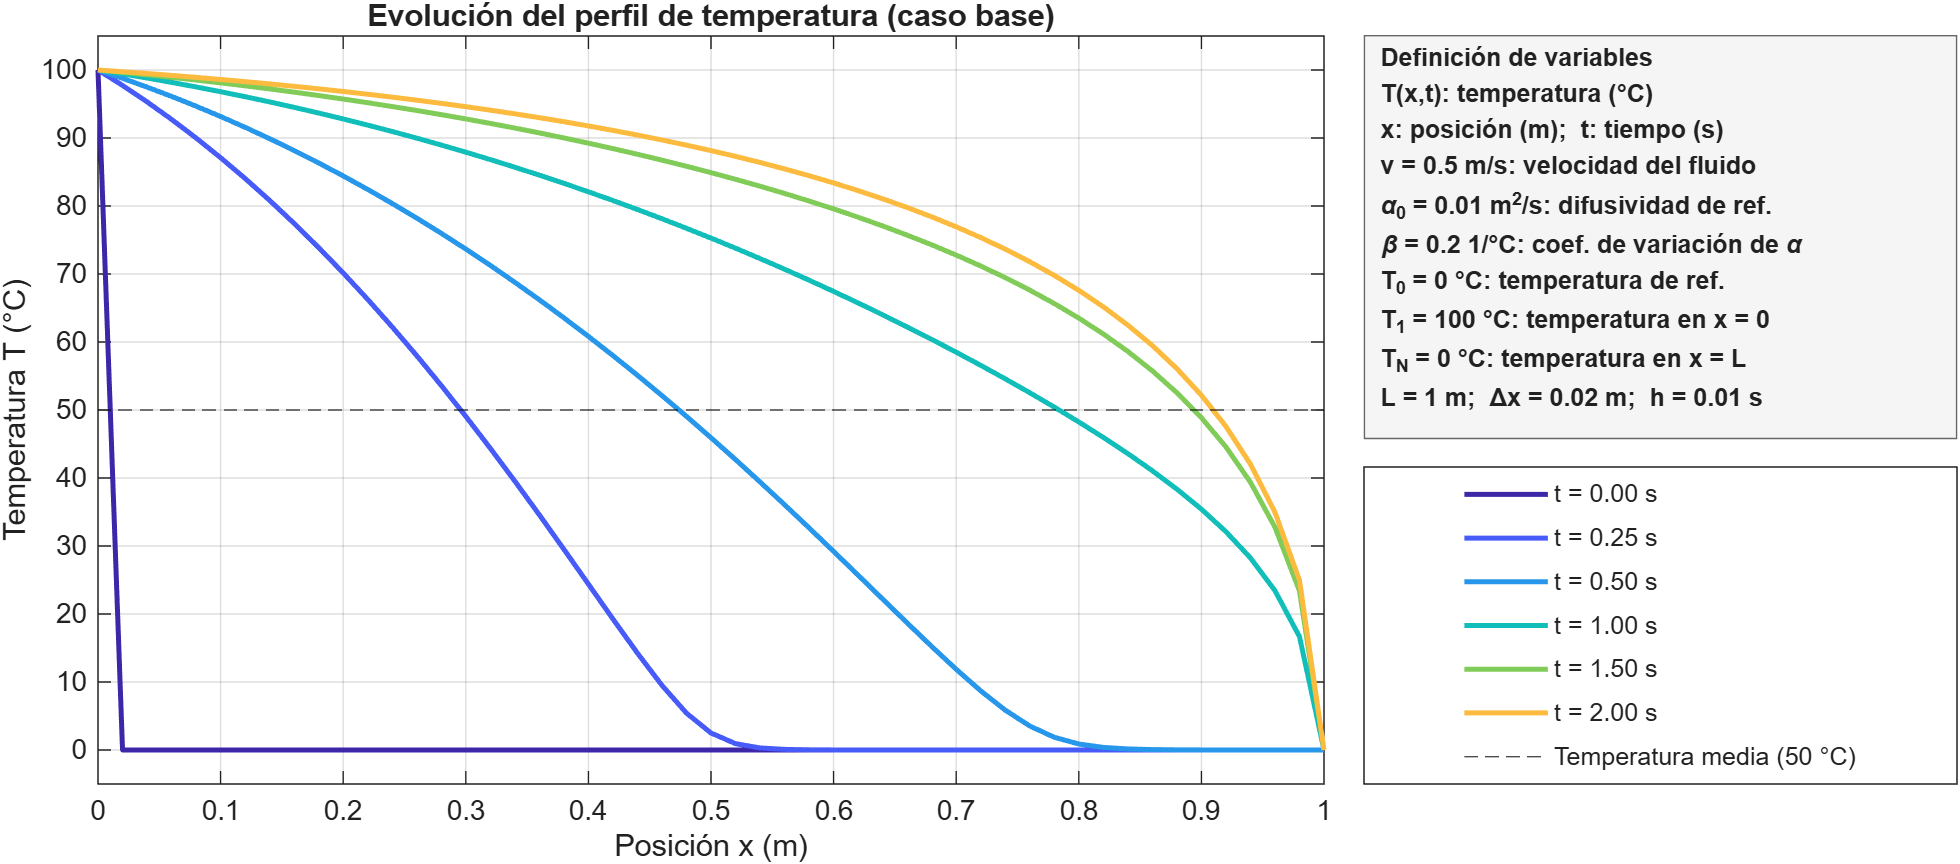
\includegraphics[width=0.9\textwidth]{fig_evolucion.png}\par
\footnotesize\textit{Nota.} Resultado con los parámetros de la Tabla~\ref{tab:parametros}. El recuadro de la derecha define las variables y la leyenda indica el instante de cada curva. La línea discontinua marca la temperatura media de 50~\textdegree C.
\end{figure*}

Para el cuarto objetivo, la posición del frente, calculada en cada instante guardado, se presenta en la Tabla~\ref{tab:frente}. El frente avanzó cada vez menos entre instantes consecutivos: su velocidad media pasó de 1,1~m/s entre 0 y 0,25~s a 0,6~m/s entre 0,5 y 1~s, y a solo 0,03~m/s entre 1,5 y 2~s.

\begin{table}[H]
\centering
\small
\refstepcounter{table}{\noindent\small\textbf{Tabla~\thetable}\label{tab:frente}\par}\vspace{1pt}
\textit{Posición del frente del caso base en el tiempo}\par\vspace{2pt}
\begin{tabular}{@{}cc@{}}
\toprule
$t$ (s) & $x_f$ (m) \\
\midrule
0    & 0,010 \\
0,25 & 0,296 \\
0,5  & 0,474 \\
1,0  & 0,784 \\
1,5  & 0,894 \\
2,0  & 0,909 \\
\bottomrule
\end{tabular}
\par\vspace{2pt}\footnotesize\textit{Nota.} $x_f$ es el punto donde $T=50$~\textdegree C, con interpolación lineal. En $t=0$ el frente queda en el primer intervalo de la malla.
\end{table}

La Figura~\ref{fig:terminos} separó la rapidez de cambio de la temperatura, $\partial T/\partial t$, en su parte advectiva y su parte difusiva en $t=1$~s. El término advectivo fue positivo en todo el dominio (36,6~\textdegree C/s en $x=0{,}5$~m) y el difusivo fue negativo y mucho menor en el centro del dominio ($-5{,}8$~\textdegree C/s en $x=0{,}5$~m). Ambos crecieron en valor absoluto cerca de la pared, donde alcanzaron cerca de $+293$ y $-264$~\textdegree C/s, y la suma, $\partial T/\partial t$, tuvo su máximo, 58~\textdegree C/s, en $x=0{,}84$~m.

\begin{figure*}[!t]
\centering
\refstepcounter{figure}{\noindent\small\textbf{Figura~\thefigure}\label{fig:terminos}\par}\vspace{1pt}
{\noindent\small\textit{Términos advectivo y difusivo de $\partial T/\partial t$ en $t=1$~s}\par}\vspace{3pt}
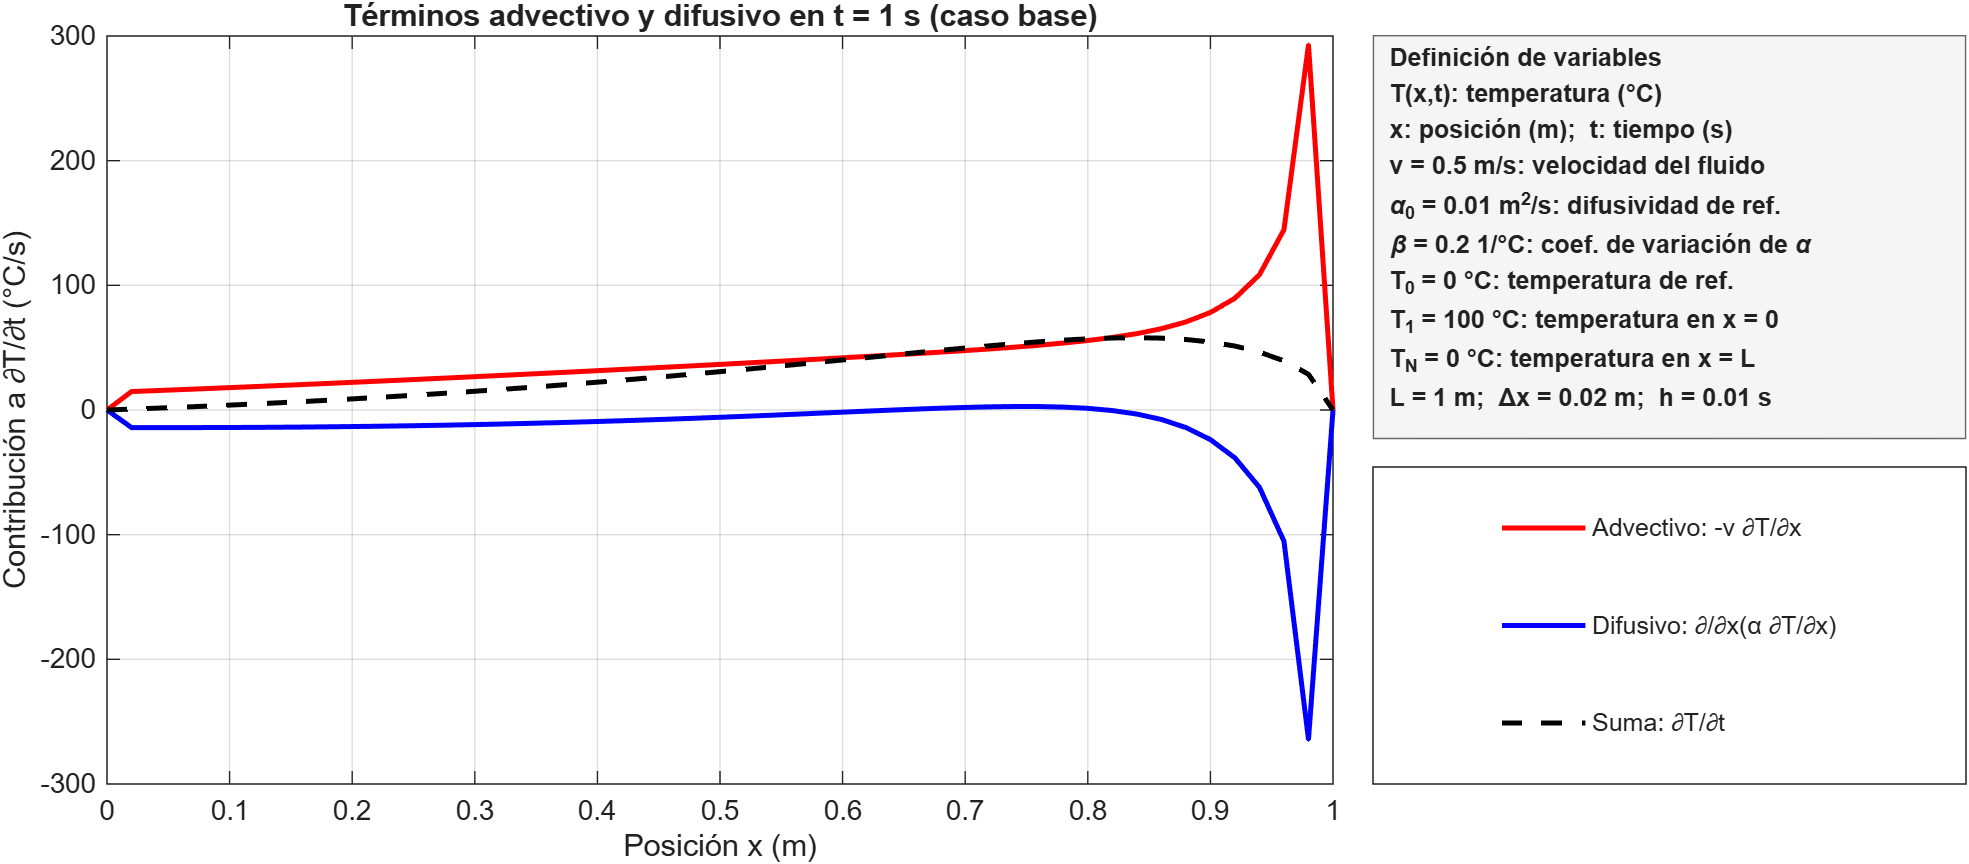
\includegraphics[width=0.9\textwidth]{fig_terminos.png}\par
\footnotesize\textit{Nota.} Caso base de la Tabla~\ref{tab:parametros}. La curva roja es $-v\,\partial T/\partial x$, la azul es $\partial(\alpha\,\partial T/\partial x)/\partial x$ y la negra discontinua es su suma, $\partial T/\partial t$, evaluadas con el esquema de la ecuación~\eqref{eq:f_semidiscreta}.
\end{figure*}

Para el tercer objetivo, primero se varió la velocidad (Figura~\ref{fig:barridov} y Tabla~\ref{tab:barridos}, panel A). Con $v=0$ el frente llegó a $x_f=0{,}598$~m en $t=2{,}0$~s, y al aumentar $v$ quedó cada vez más cerca de la pared: 0,831; 0,909 y 0,956~m. Las iteraciones de Newton-Raphson (de 2838 a 2511) y de Gauss-Seidel (cerca de 30000) cambiaron poco con $v$. Luego se varió $\beta$ (Tabla~\ref{tab:barridos}, panel B): la posición del frente disminuyó de forma monótona de 0,968~m ($\beta=0$) a 0,869~m ($\beta=0{,}4$~1/\textdegree C). Newton-Raphson necesitó 2000 iteraciones en el caso lineal y entre 2510 y 2708 en los no lineales, sin una tendencia clara, mientras que las iteraciones de Gauss-Seidel crecieron de 7509 a 44864 y el tiempo de cómputo de 17 a 44~ms.

\begin{figure*}[!t]
\centering
\refstepcounter{figure}{\noindent\small\textbf{Figura~\thefigure}\label{fig:barridov}\par}\vspace{1pt}
{\noindent\small\textit{Efecto de la velocidad $v$ sobre el perfil de temperatura en $t=2{,}0$~s}\par}\vspace{3pt}
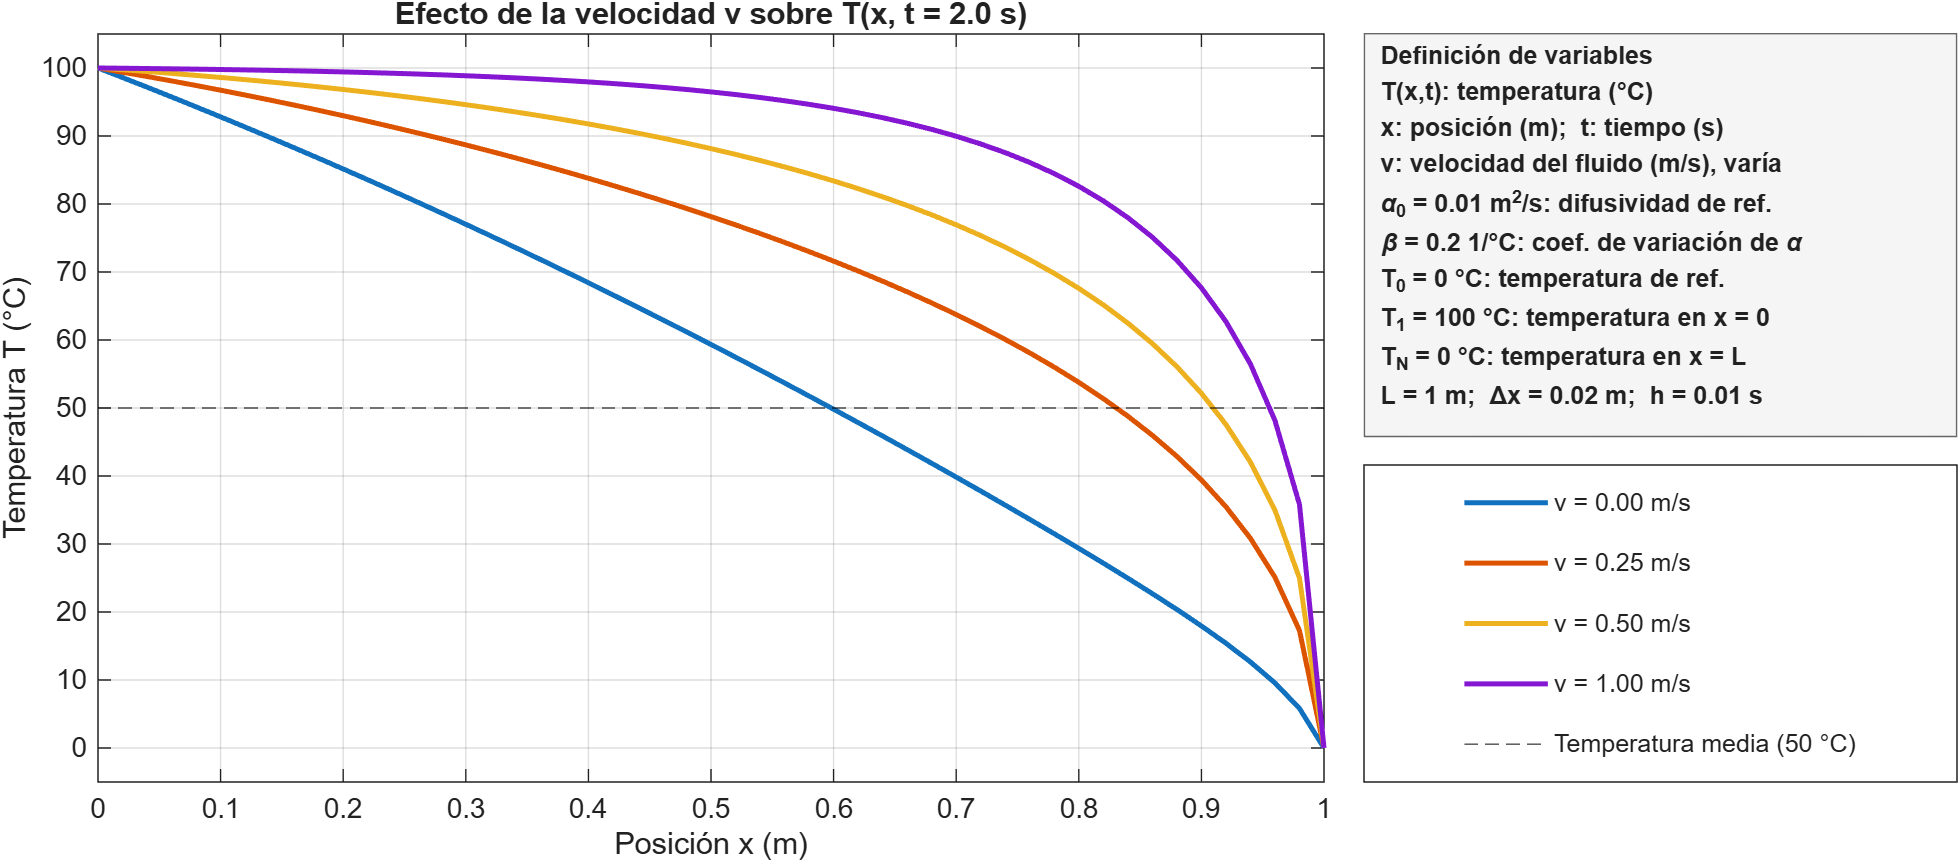
\includegraphics[width=0.9\textwidth]{fig_barrido_v.png}\par
\footnotesize\textit{Nota.} Los demás parámetros son los de la Tabla~\ref{tab:parametros}. La curva azul ($v=0$) es difusión pura; el caso base es $v=0{,}5$~m/s.
\end{figure*}

\begin{table}[H]
\centering
\small
\refstepcounter{table}{\noindent\small\textbf{Tabla~\thetable}\label{tab:barridos}\par}\vspace{1pt}
\textit{Resultados de los barridos de $v$ y de $\beta$ en $t=2{,}0$~s}\par\vspace{2pt}
\begin{tabular}{@{}ccccc@{}}
\toprule
Valor & $x_f$ (m) & Iter. N-R & Iter. G-S & Tiempo (ms) \\
\midrule
\multicolumn{5}{@{}l}{\textit{Panel A. Velocidad $v$ (m/s)}} \\
0    & 0,598 & 2838 & 29928 & 81 \\
0,25 & 0,831 & 2704 & 30975 & 72 \\
0,5  & 0,909 & 2629 & 31261 & 56 \\
1,0  & 0,956 & 2511 & 30363 & 37 \\
\midrule
\multicolumn{5}{@{}l}{\textit{Panel B. Coeficiente $\beta$ (1/\textdegree C)}} \\
0   & 0,968 & 2000 & 7509  & 17 \\
0,1 & 0,937 & 2708 & 22638 & 31 \\
0,2 & 0,909 & 2629 & 31261 & 36 \\
0,4 & 0,869 & 2510 & 44864 & 44 \\
\bottomrule
\end{tabular}
\par\vspace{2pt}\footnotesize\textit{Nota.} $x_f$ es la posición del frente. N-R: Newton-Raphson; G-S: Gauss-Seidel. El tiempo de cómputo depende del equipo y varía entre ejecuciones.
\end{table}

Finalmente, la Tabla~\ref{tab:convergencia} presentó el error máximo frente a la solución de referencia al variar los pasos espacial y temporal. Al reducir $\Delta x$ de 0,04 a 0,005~m, el error máximo bajó de 1,16 a 0,056~\textdegree C, con órdenes de convergencia observados de 1,2; 1,4 y 1,8, y las iteraciones de Gauss-Seidel subieron de 15568 a 264489. Al reducir $h$ de 0,04 a 0,005~s, el error máximo bajó de $3{,}9\times10^{-5}$ a $1{,}4\times10^{-6}$~\textdegree C, con órdenes observados de 1,3; 1,5 y 2,0; las iteraciones de Newton-Raphson subieron de 790 a 4917, mientras que las de Gauss-Seidel subieron solo de 25402 a 38758.

\begin{table}[H]
\centering
\small
\refstepcounter{table}{\noindent\small\textbf{Tabla~\thetable}\label{tab:convergencia}\par}\vspace{1pt}
\textit{Error máximo e iteraciones al variar los pasos espacial y temporal}\par\vspace{2pt}
\begin{tabular}{@{}cccccc@{}}
\toprule
Paso & $e_{\max}$ (\textdegree C) & Orden & N-R & G-S \\
\midrule
\multicolumn{5}{@{}l}{\textit{Panel A. Paso espacial $\Delta x$ (m), con $h=0{,}01$~s}} \\
0,04  & $1{,}16$ & --- & 2613 & 15568 \\
0,02  & $0{,}502$ & 1,2 & 2629 & 31261 \\
0,01  & $0{,}193$ & 1,4 & 2644 & 83725 \\
0,005 & $0{,}056$ & 1,8 & 2649 & 264489 \\
\midrule
\multicolumn{5}{@{}l}{\textit{Panel B. Paso de tiempo $h$ (s), con $\Delta x=0{,}02$~m}} \\
0,04  & $3{,}9\times10^{-5}$ & --- & 790 & 25402 \\
0,02  & $1{,}6\times10^{-5}$ & 1,3 & 1421 & 27407 \\
0,01  & $5{,}6\times10^{-6}$ & 1,5 & 2629 & 31261 \\
0,005 & $1{,}4\times10^{-6}$ & 2,0 & 4917 & 38758 \\
\bottomrule
\end{tabular}
\par\vspace{2pt}\footnotesize\textit{Nota.} $e_{\max}$ es el error máximo en $t=2{,}0$~s frente a la solución de referencia. Orden $=\log_2(e_{\max}^{\text{anterior}}/e_{\max})$. N-R y G-S: iteraciones totales de Newton-Raphson y de Gauss-Seidel.
\end{table}

En síntesis, el esquema convergió en todas las etapas y en todas las corridas. El caso base tuvo un error máximo de 0,50~\textdegree C y el frente alcanzó $x_f=0{,}909$~m en 2,0~s, con una velocidad de avance que se redujo casi a cero al llegar a la pared. La posición del frente aumentó con $v$ y disminuyó con $\beta$; el error máximo disminuyó al reducir $\Delta x$ y $h$; y las iteraciones de Gauss-Seidel crecieron con $\beta$ y con el refinamiento espacial.

\section{Discusión}
\label{sec:discusion}

La convergencia del esquema en todas las etapas (objetivo i) es coherente con la combinación elegida. Newton-Raphson necesitó pocas iteraciones por etapa (Sección~\ref{sec:resultados}), lo esperable cuando la aproximación inicial, que es la etapa anterior, está cerca de la solución \citep{Deuflhard1974}, y Gauss-Seidel convergió en todos los casos, lo que es consistente con que la matriz $\mathbf{I}-h\gamma\mathbf{J}_f$ sea diagonalmente dominante con $v\,\Delta x/\alpha\le 2$ \citep{Zhang2015}. Los perfiles de la Figura~\ref{fig:evolucion} fueron monótonos y sin oscilaciones, lo que coincide con lo descrito por \citet{Gresho1981}: las diferencias centradas producen oscilaciones cuando el número de Péclet de celda supera 2, y en el caso base vale 1. Con ello el esquema resuelve el transporte de calor sin recurrir a un término de estabilización, a diferencia de lo que sugerirían velocidades mayores con la misma malla.

El error máximo del caso base, 0,50~\textdegree C (objetivo ii), se ubicó en la capa límite junto a la pared (Figura~\ref{fig:evolucion}, $x=0{,}98$~m), donde el perfil pasa de 25 a 0~\textdegree C en un solo intervalo de la malla. Esto es esperable porque el espesor de esa capa es del orden de $\alpha_0/v=0{,}02$~m, igual a $\Delta x$, de modo que la malla base apenas la resuelve. Por la misma razón, el orden de convergencia espacial observado en la Tabla~\ref{tab:convergencia} (1,2 a 1,8) fue menor que el orden dos de las diferencias finitas empleadas y se acercó a él al refinar la malla, cuando la capa límite quedó mejor resuelta. En el tiempo, el error ($\le 4\times10^{-5}$~\textdegree C) fue mucho menor que el espacial, de modo que la precisión del caso base la limita la malla y no el paso de tiempo. Los órdenes temporales observados (1,3 a 2,0) fueron inferiores al orden cuatro de SDIRK4 que reportan \citet{Deng2015}; una explicación posible, que no se verificó por separado, es que el escalón de la condición inicial no es una función suave y que, con $h$ pequeño, el error ($1{,}4\times10^{-6}$~\textdegree C) ya es comparable con la tolerancia de Newton-Raphson ($10^{-6}$). Además, como la referencia usa el mismo esquema, el error medido mide su convergencia y no su exactitud absoluta.

Sobre la robustez (objetivo iii), la posición del frente aumentó con $v$ (Figura~\ref{fig:barridov} y Tabla~\ref{tab:barridos}), como corresponde a un término advectivo que empuja la temperatura hacia la pared. La Figura~\ref{fig:terminos} muestra cómo actúa ese término: fue positivo en todo el dominio y mayor que el difusivo, de modo que la temperatura de cada punto cambió sobre todo por la afectación advectiva, y la difusión la frenó parcialmente. Con $v=0$, en cambio, el frente alcanzó $0{,}598$~m solo por difusión, un valor alto que se debe a que $\alpha(100~\text{\textdegree C})=21\,\alpha_0$. Este resultado va en el sentido de lo señalado por \citet{Wang2022} y \citet{Filipov2023}: suponer la difusividad constante cambia de forma apreciable la descripción cuando los cambios de temperatura son grandes; aquí, con $\beta=0$, el frente quedó en $0{,}968$~m, $0{,}10$~m más lejos que con $\beta=0{,}4$ (Tabla~\ref{tab:barridos}). Una posible explicación de que $\beta$ acerque el frente a la corriente caliente es que una difusividad mayor en la zona caliente suaviza el perfil desde el lado de $x=0$; esta explicación no se verificó por separado. En cuanto al costo, las iteraciones de Gauss-Seidel crecieron con $\beta$ y al refinar $\Delta x$ (Tablas~\ref{tab:barridos} y~\ref{tab:convergencia}), mientras que casi no cambiaron con $v$. Esto es consistente con la teoría clásica de las iteraciones de Gauss-Seidel en problemas elípticos \citep{Young1954}: cuanto más se parece el sistema a un problema de difusión puro, con más difusividad o con una malla más fina, más lenta es la convergencia.

Sobre la aplicación (objetivo iv), la Tabla~\ref{tab:frente} muestra que el frente avanza con rapidez al inicio y casi se detiene al acercarse a la pared. Esto se explica porque la pared se mantiene a 0~\textdegree C (condición de Dirichlet): el perfil deja de desplazarse y se aproxima a una forma casi estacionaria, con una capa límite junto a la pared donde el término advectivo y el difusivo casi se compensan (Figura~\ref{fig:terminos}). Por eso, a diferencia de la advección pura, que llevaría el frente a $x=L$ en $L/v=2$~s, el frente de 50~\textdegree C quedó en 0,909~m.

Las limitaciones del estudio influyeron en estos resultados. El modelo es unidimensional y con velocidad constante, de modo que no representa la capa límite ni la estela reales del cilindro; el caso base es sintético, con una difusividad mucho mayor que la de fluidos reales, por lo que los valores absolutos no son extrapolables y el análisis cualitativo es el que tiene alcance general. La referencia se obtuvo con el mismo esquema y no existe una solución analítica con la cual contrastarla, y los barridos cubrieron solo un instante final y un parámetro a la vez. Aun así, el esquema mostró un costo bajo (0,13~s para el caso base) y resultados coherentes con lo esperado para la combinación de un método implícito, Newton-Raphson y Gauss-Seidel.

\section{Conclusiones}
\label{sec:conclusiones}

Se modeló numéricamente el transporte transitorio de calor unidimensional con advección y difusividad térmica variable, y se analizó el avance del frente de temperatura entre una corriente caliente y la pared de un tubo cilíndrico, por lo que se cumplió el objetivo general. La combinación de diferencias finitas, SDIRK4, Newton-Raphson y Gauss-Seidel convergió en todas las etapas (primer objetivo específico); el caso base tuvo un error máximo de 0,50~\textdegree C frente a la solución de referencia, concentrado en la capa límite de la pared (segundo); el error disminuyó al reducir los pasos espacial y temporal, la velocidad desplazó el frente hacia la pared y el coeficiente de variación de la difusividad lo acercó a la corriente caliente, mientras que las iteraciones de Gauss-Seidel crecieron con la no linealidad y con el refinamiento espacial (tercero); y el frente alcanzó 0,909~m en 2,0~s, con una velocidad de avance que disminuyó hasta casi detenerse (cuarto).

El estudio aporta un modelo claro y reproducible para el transporte transitorio de calor con difusividad variable, que separa la contribución de los términos advectivo y difusivo, y cuantifica la precisión, la robustez y el costo de la combinación de un método implícito de cuarto orden con un método para la no linealidad y un método iterativo lineal. Su alcance es el de un modelo unidimensional con velocidad constante y parámetros sintéticos, y su relevancia está en que el mismo esquema se puede usar para estudiar cómo la dependencia de las propiedades térmicas con la temperatura modifica el transporte de calor en un flujo.

% ==================== BIBLIOGRAFÍA ====================

\begin{thebibliography}{19}

\bibitem[Alexander(1977)]{Alexander1977}
Alexander, R. (1977). Diagonally implicit Runge--Kutta methods for stiff O.D.E.'s. \textit{SIAM Journal on Numerical Analysis, 14}(6), 1006--1021. \url{https://doi.org/10.1137/0714068}

\bibitem[Ascher et al.(1997)]{Ascher1997}
Ascher, U. M., Ruuth, S. J., \& Spiteri, R. J. (1997). Implicit-explicit Runge-Kutta methods for time-dependent partial differential equations. \textit{Applied Numerical Mathematics, 25}(2--3), 151--167. \url{https://doi.org/10.1016/S0168-9274(97)00056-1}

\bibitem[Bevan et al.(2016)]{Bevan2016}
Bevan, R. L. T., Boileau, E., van Loon, R., Lewis, R. W., \& Nithiarasu, P. (2016). A comparative study of fractional step method in its quasi-implicit, semi-implicit and fully-explicit forms for incompressible flows. \textit{International Journal of Numerical Methods for Heat \& Fluid Flow, 26}(3/4), 595--623. \url{https://doi.org/10.1108/HFF-06-2015-0233}

\bibitem[Boscarino et al.(2015)]{Boscarino2015}
Boscarino, S., B{\"u}rger, R., Mulet, P., Russo, G., \& Villada, L. M. (2015). Linearly implicit IMEX Runge--Kutta methods for a class of degenerate convection-diffusion problems. \textit{SIAM Journal on Scientific Computing, 37}(2), B305--B331. \url{https://doi.org/10.1137/140967544}

\bibitem[Butcher(1996)]{Butcher1996}
Butcher, J. C. (1996). A history of Runge-Kutta methods. \textit{Applied Numerical Mathematics, 20}(3), 247--260. \url{https://doi.org/10.1016/0168-9274(95)00108-5}

\bibitem[Deng y Pan(2015)]{Deng2015}
Deng, D., \& Pan, T. (2015). A fourth-order singly diagonally implicit Runge-Kutta method for solving one-dimensional Burgers' equation. \textit{IAENG International Journal of Applied Mathematics, 45}(4), Article IJAM\_45\_4\_11. \url{https://www.iaeng.org/IJAM/issues_v45/issue_4/IJAM_45_4_11.pdf}

\bibitem[Deng et al.(2014)]{Deng2014}
Deng, Z., Sun, Y., Li, F., \& Rizwan-uddin. (2014). Application of diagonally implicit Runge-Kutta method for solving time-dependent convection-diffusion equation. \textit{Nuclear Power Engineering, 35}(1), 5--9.

\bibitem[Deuflhard(1974)]{Deuflhard1974}
Deuflhard, P. (1974). A modified Newton method for the solution of ill-conditioned systems of nonlinear equations with application to multiple shooting. \textit{Numerische Mathematik, 22}(4), 289--315. \url{https://doi.org/10.1007/BF01406969}

\bibitem[Ejaz et al.(2024)]{Ejaz2024}
Ejaz, S. T., Malik, S., Younis, J., Sellami, R., \& Alnefaie, K. (2024). An innovative subdivision collocation algorithm for heat conduction equation with non-uniform thermal diffusivity. \textit{Scientific Reports, 14}(1). \url{https://doi.org/10.1038/s41598-024-73772-3}

\bibitem[Filipov et al.(2023)]{Filipov2023}
Filipov, S. M., Hristov, J., Avdzhieva, A., \& Farag{\'o}, I. (2023). A coupled PDE-ODE model for nonlinear transient heat transfer with convection heating at the boundary: Numerical solution by implicit time discretization and sequential decoupling. \textit{Axioms, 12}(4), Article 323. \url{https://doi.org/10.3390/axioms12040323}

\bibitem[Gresho y Lee(1981)]{Gresho1981}
Gresho, P. M., \& Lee, R. L. (1981). Don't suppress the wiggles---They're telling you something! \textit{Computers \& Fluids, 9}(2), 223--253. \url{https://doi.org/10.1016/0045-7930(81)90026-8}

\bibitem[Kennedy y Carpenter(2003)]{Kennedy2003}
Kennedy, C. A., \& Carpenter, M. H. (2003). Additive Runge--Kutta schemes for convection--diffusion--reaction equations. \textit{Applied Numerical Mathematics, 44}(1--2), 139--181. \url{https://doi.org/10.1016/S0168-9274(02)00138-1}

\bibitem[Lev{\'y} y May(2022)]{Levy2022}
Lev{\'y}, T., \& May, G. (2022). Comparison of implicit time-discretization schemes for hybridized discontinuous Galerkin methods. \textit{Applied and Computational Mechanics, 16}(2). \url{https://doi.org/10.24132/acm.2022.786}

\bibitem[Mt Aznam et al.(2019)]{MtAznam2019}
Mt Aznam, S., Che Ghani, N. A., \& Chowdhury, M. S. H. (2019). A numerical solution for nonlinear heat transfer of fin problems using the Haar wavelet quasilinearization method. \textit{Results in Physics, 14}, Article 102393. \url{https://doi.org/10.1016/j.rinp.2019.102393}

\bibitem[Singh et al.(2024)]{Singh2024}
Singh, R., Singh, J., Kumar, R., \& Gupta, M. (2024). Computational fluid dynamics of flow over a cylindrical tube for steady and transient flow conditions. \textit{International Journal on Interactive Design and Manufacturing}. Advance online publication. \url{https://doi.org/10.1007/s12008-024-01970-4}

\bibitem[Wang et al.(2022)]{Wang2022}
Wang, F., Liu, Y.-C., \& Zheng, H. (2022). A localized method of fundamental solution for numerical simulation of nonlinear heat conduction. \textit{Mathematics, 10}(5), Article 773. \url{https://doi.org/10.3390/math10050773}

\bibitem[Young(1954)]{Young1954}
Young, D. (1954). Iterative methods for solving partial difference equations of elliptic type. \textit{Transactions of the American Mathematical Society, 76}(1), 92--111. \url{https://doi.org/10.1090/S0002-9947-1954-0059635-7}

\bibitem[Ypma(1995)]{Ypma1995}
Ypma, T. J. (1995). Historical development of the Newton--Raphson method. \textit{SIAM Review, 37}(4), 531--551. \url{https://doi.org/10.1137/1037125}

\bibitem[Zhang et al.(2015)]{Zhang2015}
Zhang, C.-Y., Ye, D., Zhong, C.-L., \& Luo, S. (2015). Convergence on Gauss-Seidel iterative methods for linear systems with general H-matrices. \textit{The Electronic Journal of Linear Algebra, 30}, 843--870. \url{https://doi.org/10.13001/1081-3810.1972}

\end{thebibliography}

\clearpage
\section*{Anexos}
\textbf{Repositorio del código.} Los archivos \texttt{.mlx} de la implementación (programa principal \texttt{main.mlx} y funciones en la carpeta \texttt{funciones}), con su versión en texto plano \texttt{.m}, están disponibles en el repositorio en la nube:

\url{https://github.com/jeffHQ/NumericMethods}

\end{document}
